
\documentclass[a4paper]{article}
\usepackage[utf8]{inputenc}

\usepackage[english,german]{babel} 
\usepackage[utf8]{inputenc}

\usepackage{alltt}
\usepackage{amsmath}
\usepackage{amssymb}
\usepackage{amsthm}
\usepackage{color}
\usepackage{enumitem}
\usepackage{epsfig}
\usepackage{fancyhdr}
\usepackage{float}
\usepackage{framed}
\usepackage{graphicx} 
\usepackage{graphics}
\usepackage{hyperref}
\usepackage{listings}
\usepackage{multirow}
\usepackage{tabularx}
\usepackage{textcomp}
\usepackage{tikz}
\usepackage{url}
\usepackage{vmargin}
\usepackage{xspace}
\usepackage{comment}
\usetikzlibrary{calc,trees,positioning,arrows,chains,shapes.geometric,%
    decorations.pathreplacing,decorations.pathmorphing,shapes,%
    matrix,shapes.symbols,topaths,matrix}
\newcommand{\question}[2][0]{\section{{#2} \hfill ({#1} P.)}}
\setpapersize{A4}
\setmargins{2.5cm}{2.0cm}% % linker & oberer Rand
         {16cm}{22cm}%   % Textbreite und -hoehe
           {48pt}{36pt}%   % Kopfzeilenhoehe und -abstand
           {0pt}{30pt}%    % \footheight (egal) und Fusszeilenabstand

\frenchspacing
\pagestyle{fancy}
\sloppy

\newcommand{\hide}[1]{}

\markright{Kopfzeile}


\tikzset{
>=stealth',
  punktchain/.style={
    rectangle,
    rounded corners,
    % fill=black!10,
    draw=black, very thick,
    text width=10em,
    minimum height=3em,
    text centered,
    on chain},
  line/.style={draw, thick, <-},
  element/.style={
    tape,
    top color=white,
    bottom color=blue!50!black!60!,
    minimum width=8em,
    draw=blue!40!black!90, very thick,
    text width=10em,
    minimum height=3.5em,
    text centered,
    on chain},
  every join/.style={->, thick,shorten >=1pt},
  decoration={brace},
  tuborg/.style={decorate},
  tubnode/.style={midway, right=2pt},
}


\setlength{\parindent}{0pt}
\setlength{\parskip}{5pt}
\fboxsep1.5mm


\lstdefinestyle{mystyle}{
    backgroundcolor=\color{white},   
    commentstyle=\color{codegray},
    keywordstyle=\bf \ttfamily \color{codepurple},
    numberstyle=\tiny\color{codegray},
    stringstyle=\color{codegreen},
    basicstyle=\footnotesize,
    breakatwhitespace=false,         
    breaklines=true,                 
    captionpos=b,                    
    keepspaces=true,                 
    numbers=left,                    
    numbersep=5pt,                  
    showspaces=false,                
    showstringspaces=false,
    showtabs=false,                  
    tabsize=8,
    keepspaces,
    extendedchars=true, 
      upquote=true,
    columns=fixed,
    showstringspaces=false,
    extendedchars=true,
    breaklines=true,
    frame=single,
    showspaces=false,
    showstringspaces=false,
    rulecolor=\color{white},
}

\lstdefinelanguage{sql}[]{}{
        %tag=[s]<>,      % =*: also apply styles within tag, =**: cumulate styles
        morekeywords={sql, VIEW, AS, FROM, SELECT, WHERE, FUNCTION, BOOLEAN, RETURNS, DETERMINISTIC, RETURN, REFERENCES, WITH, SEQUENCE, TRUNCATE, START, CREATE, AS, LANGUAGE, FUNCTION, CURSOR, PREPARE, OPEN, USING, CLOSE, DECLARE, END, BEGIN, EXEC, SQL, CONNECT TO, DISCONNECT, COMMIT, LOOP, IF, THEN, ELSE, WHILE, BREAK, EXIT, INSERT, INTO, VALUES, UPDATE, SET, TABLE, PRIMARY, KEY, AND, UNION, ALL, JOIN, ON, GROUP, BY, MATERIALIZED, INT, DATE, COUNT, ORDER, OVER, PARTITION, ASC, DESC, VARCHAR, NOT, NULL, PRIMARY, KEY, DECIMAL, SUM, AVG, ROWS, BETWEEN, PRECEDING, CURRENT, ROW, INSTEAD, TRIGGER, OF, FOR, EACH, EXECUTE, PROCEDURE, DISTINCT, HAVING, LIMIT},
morestring=[s]{'}{'},
morecomment=[l]{--}
        %sensitive=false
}

\lstset{style=mystyle,numbers=none,basicstyle=\ttfamily,upquote=true}

 
\definecolor{codegreen}{rgb}{0,0.6,0}
\definecolor{codegray}{rgb}{0.5,0.5,0.5}
\definecolor{codepurple}{rgb}{0.38,0,0.72}
\definecolor{backcolour}{rgb}{0.95,0.95,0.92}
\definecolor{backcolourSingleCode}{rgb}{0.95,0.95,0.92}

\newcommand{\subtitle}{\textbf{Exercise 7}}
\newcommand{\outdate}{04.12.2023}
\newcommand{\duedate}{11.12.2023 12:00 MEZ}
\newcommand{\video}{036}

\usepackage{tkz-euclide}
\begin{document}

\lhead{\begin{tabular}{l}
{\bf Database Systems WS 2023/24}\\
{\bf \subtitle: Distributed \outdate, Due \duedate}\\
{Submitted by }
\end{tabular}
}
\rhead{}

\question[1]{Space filling curves for NN-queries}
\begin{enumerate}
  \item 
  Implement space-filling z-curves in a language of your choice.
Your program has to take two files which contain points as input.
The first file contains all the points of the base data set, while the second file contains query points.
The program has to calculate and display:
\begin{itemize}
\item The k-NN, of each query point, in the base data set, based on the actual distance.
\item The k-NN, of each query point, in the base data set, based on the z-curve distance.
\end{itemize}

You can use the template in OLAT, which already parses the files and provides utility classes.
Submit the code and the output of your program when executed with $k = 3$ and the two data files provided in OLAT.
If you do not use the template, also submit instructions on how to compile and execute your program.

\textit{Note: } If you use code from external sources, provide the source as a comment.\\

{\bf Solution:}\\
\begin{figure}[H]
  \centering
  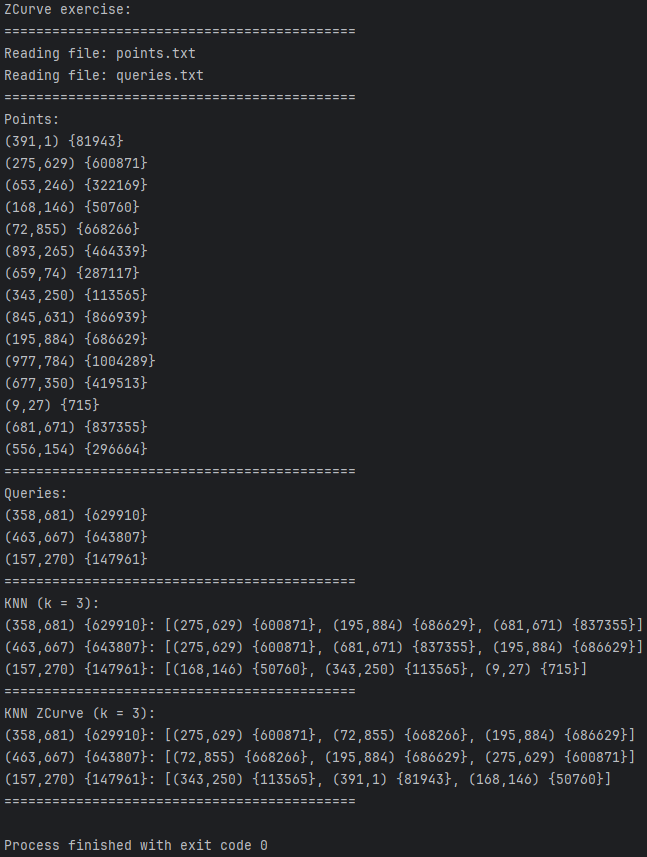
\includegraphics[scale = 0.6]{ZCurveOutput.PNG}
\end{figure}

\item
Which differences can you see between the two results of your implementation?
Explain why are or why are not the results the same.\\\\
{\bf Solution:}\\
Some of the actual k-NN are matching the k-NN according to the z-curve value, but not all of them.
The z-curve mapping is only an approximation of the actual k-NN.\\

Let's have a look at the points $A(0,0)$, $B(1,0)$, and $C(0,1)$. The real distance between $A$ and $B$ is $1$.
Also, the z-value is $1$ in this case. The real distance between $A$ and $C$ is also $1$, but in this case, 
the z-value is $2$. Because of the shape of the z-curve, the z-value is only an estimation of the real distance.

\end{enumerate}

\question[1]{R Tree}

Given the following two-dimensional objects:

\begin{center}
  \begin{tikzpicture}

    \draw[help lines, color=gray!30, dashed] (0,0) grid (10,6);

    \draw (0,0) -- coordinate (x axis mid) (10,0);
    \draw (0,0) -- coordinate (y axis mid) (0,6);

    \foreach \x in {0,...,10} \draw (\x,1pt) -- (\x,-3pt) node[anchor=north] {\x};
    \foreach \y in {0,...,6}  \draw (1pt,\y) -- (-3pt,\y) node[anchor=east] {\y};

    \tkzDefPoint(1,1){f1a};
    \tkzDefPoint(1,5){f1b};
    \tkzDefPoint(2,5){f1c};
    \tkzDefPoint(3,3){f1d};
    \tkzDefPoint(2,1){f1e};

    \tkzDrawPolygon[fill=purple!30](f1a,f1b,f1c,f1d,f1e);
    \node at (barycentric cs:f1a=1,f1b=1,f1c=1,f1d=1,f1e=1) {F1};

    \draw[fill=yellow!30] (4,5) circle (1);
    \node at (4,5) {F2};

    \tkzDefPoint(4,2){f3a};
    \tkzDefPoint(5,3){f3b};
    \tkzDefPoint(6,3){f3c};
    \tkzDefPoint(6,2){f3d};
    \tkzDefPoint(5,1){f3e};

    \tkzDrawPolygon[fill=green!30](f3a,f3b,f3c,f3d,f3e);
    \node at (barycentric cs:f3a=1,f3b=1,f3c=1,f3d=1,f3e=1) {F3};

    \draw[fill=blue!30] (8,2) circle (1);
    \node at (8,2) {F4};

    \tkzDefPoint(6,4){f5a};
    \tkzDefPoint(9,4){f5b};
    \tkzDefPoint(9,6){f5c};
    \tkzDefPoint(8,6){f5d};
    \tkzDefPoint(8,5){f5e};
    \tkzDefPoint(6,5){f5f};

    \tkzDrawPolygon[fill=red!30](f5a,f5b,f5c,f5d,f5e,f5f);
    \node at (barycentric cs:f5a=3,f5b=3,f5c=1,f5d=1,f5e=1,f5f=1) {F5};
  \end{tikzpicture}
\end{center}

For the following R tree operations, explain exactly which steps are performed:

\begin{enumerate}
\item
  {\em Store the objects F1, F2, F3, F4, F5 in an initially empty R tree}.
  One node fits 1--2 entries.\\\\
  {\bf Solution:}\\
  The objects get inserted one after the other; in theory, they can be inserted in any node. 
  I decided for the following insertion order: F1, F5, F4, F2, F3. F1 and F5 get inserted into the tree.\\
\begin{center}
  \begin{tikzpicture}[level distance=1.5cm,
    level 1/.style={sibling distance=3cm}]
    \node[draw]{$R1|R2$}
      child{node[draw]{$F1|null$}}
      child{node[draw]{$F5|null$}};
  \end{tikzpicture}
\end{center}
  

R1 is the smallest rectangle that fits around F1, and R2 is the smallest rectangle that fits around F5. Insertion of F4:\\
Calculate the area differences of R1 if F4 gets inserted into R1 and calculate the area difference of R2 if F4 gets inserted.\\\\
  \begin{center}
    $A_{R1} = 8 \cdot 4 - 2 \cdot 4 = 24$\\
    $A_{R2} = 5 \cdot 3 - 6 \cdot 4 = 9$
  \end{center}
    
  Insert F4 int R2 because the area increase is smaller then when inserted into R2\\\\
  \begin{center}
    \begin{tikzpicture}[level distance=1.5cm,
      level 1/.style={sibling distance=3cm}]
      \node[draw]{$R1|R2$}
        child{node[draw]{$F1|null$}}
        child{node[draw]{$F5|F4$}};
    \end{tikzpicture}
  \end{center}
  Insertion of F2:\\
  Calculate the area differences of R1 if F2 gets inserted into R1 and calculate the area difference of R2 if F2 gets inserted.\\\\
  \begin{center}
    $A_{R1} = 4 \cdot 5 - 2 \cdot 4 = 12$\\
    $A_{R2} = 5 \cdot 3 - 3 \cdot 5 = 15$
  \end{center}
    
  Insert F2 int R1 because the area increase is smaller then when inserted into R1\\\\
  \begin{center}
    \begin{tikzpicture}[level distance=1.5cm,
      level 1/.style={sibling distance=3cm}]
      \node[draw]{$R1|R2$}
        child{node[draw]{$F1|F2$}}
        child{node[draw]{$F5|F4$}};
    \end{tikzpicture}
  \end{center}
  Insertion of F3:\\
  Calculate the area differences of R1 if F2 gets inserted into R1 and calculate the area difference of R2 if F2 gets inserted.\\\\
  \begin{center}
    $A_{R1} = 5 \cdot 5 - 4 \cdot 5 = 5$\\
    $A_{R2} = 5 \cdot 5 - 3 \cdot 5 = 10$
  \end{center}
  Insert F2 int R1 because the area increase is smaller then when inserted into R1. The maximum of objects in R1 is already reached. 
  In order to insert F2 R1 needs to be split into two rectangles. The size of the two newly created rectangles R3 and R4 should be minimal in the optimal case.\\
  Calculation of the area of all possible split combinations:\\\\
  \begin{center}
    $R3[F1, F2], R4[F3]$ $A = 4 \cdot 5 + 2 \cdot 2 = 24$\\
    $R3[F1, F3], R4[F2]$ $A = 5 \cdot 4 + 2 \cdot 2 = 24$\\
    $R3[F3, F2], R4[F1]$ $A = 3 \cdot 5 + 2 \cdot 4 = 23$
  \end{center}
    
    According to the Calculation the last option is to optimal one because the area of R3 and R4 will be minimal. The R-Tree looks now like:\\\\
    \begin{center}
      \begin{tikzpicture}[level distance=1.5cm,
        level 1/.style={sibling distance=3cm},
        level 2/.style={sibling distance=3cm}]
        \node[draw]{$R1|R2$}
          child
          { node[draw]{$R3|R4$}
            child{node[draw]{$F3|F2$}}
            child{node[draw]{$F1|null$}}
          }
          child{node[draw]{$F5|F4$}};
      \end{tikzpicture}
    \end{center}
    
    In the two dimensional plane the R-Tree looks like the following:
    \begin{center}
      \begin{tikzpicture}
    
        \draw[help lines, color=gray!30, dashed] (0,0) grid (10,6);
    
        \draw (0,0) -- coordinate (x axis mid) (10,0);
        \draw (0,0) -- coordinate (y axis mid) (0,6);
    
        \foreach \x in {0,...,10} \draw (\x,1pt) -- (\x,-3pt) node[anchor=north] {\x};
        \foreach \y in {0,...,6}  \draw (1pt,\y) -- (-3pt,\y) node[anchor=east] {\y};
    
        \tkzDefPoint(1,1){f1a};
        \tkzDefPoint(1,5){f1b};
        \tkzDefPoint(2,5){f1c};
        \tkzDefPoint(3,3){f1d};
        \tkzDefPoint(2,1){f1e};
    
        
        \tkzDrawPolygon[fill=purple!30](f1a,f1b,f1c,f1d,f1e);
        \node at (barycentric cs:f1a=1,f1b=1,f1c=1,f1d=1,f1e=1) {F1};
    
        \draw[fill=yellow!30] (4,5) circle (1);
        \node at (4,5) {F2};
    
        \tkzDefPoint(4,2){f3a};
        \tkzDefPoint(5,3){f3b};
        \tkzDefPoint(6,3){f3c};
        \tkzDefPoint(6,2){f3d};
        \tkzDefPoint(5,1){f3e};
    
        \tkzDrawPolygon[fill=green!30](f3a,f3b,f3c,f3d,f3e);
        \node at (barycentric cs:f3a=1,f3b=1,f3c=1,f3d=1,f3e=1) {F3};
    
        \draw[fill=blue!30] (8,2) circle (1);
        \node at (8,2) {F4};
    
        \tkzDefPoint(6,4){f5a};
        \tkzDefPoint(9,4){f5b};
        \tkzDefPoint(9,6){f5c};
        \tkzDefPoint(8,6){f5d};
        \tkzDefPoint(8,5){f5e};
        \tkzDefPoint(6,5){f5f};
    
        \tkzDrawPolygon[fill=red!30](f5a,f5b,f5c,f5d,f5e,f5f);
        \node at (barycentric cs:f5a=3,f5b=3,f5c=1,f5d=1,f5e=1,f5f=1) {F5};

        \tkzDefPoint(1,1){R1a};
        \tkzDefPoint(6,1){R1b};
        \tkzDefPoint(6,6){R1c};
        \tkzDefPoint(1,6){R1d};
    
        \tkzDrawPolygon[line width=0.6mm, red](R1a, R1b, R1c, R1d);
        \node at (2,5.5) {\textcolor{red}{R1}};

        \tkzDefPoint(6,1){R2a};
        \tkzDefPoint(9,1){R2b};
        \tkzDefPoint(9,6){R2c};
        \tkzDefPoint(6,6){R2d};
    
        \tkzDrawPolygon[line width=0.6mm, red](R2a, R2b, R2c, R2d);
        \node at (7,5.5) {\textcolor{red}{R2}};

        \tkzDefPoint(3,1){R3a};
        \tkzDefPoint(6,1){R3b};
        \tkzDefPoint(6,6){R3c};
        \tkzDefPoint(3,6){R3d};
    
        \tkzDrawPolygon[line width=0.2mm, green](R3a, R3b, R3c, R3d);
        \node at (5.5,5.5) {\textcolor{green}{R3}};

        \tkzDefPoint(1,1){R4a};
        \tkzDefPoint(3,1){R4b};
        \tkzDefPoint(3,5){R4c};
        \tkzDefPoint(1,5){R4d}; 
    
        \tkzDrawPolygon[line width=0.2mm, green](R4a, R4b, R4c, R4d);
        \node at (2.6,4.5) {\textcolor{green}{R4}};
      \end{tikzpicture}
    \end{center}
\item
  {\em Find all objects, containing the point (6,2).}\\\\
  {\bf Solution:}\\
  Step by step execution:\\
  \subitem
  Scan the root of the tree (R1,R2)
  \subitem
  Check if (6,2) is in R1 $\Rightarrow$ true $\Rightarrow$ put R3 and R4 in the queue
  \subitem
  Check if (6,2) is in R2 $\Rightarrow$ true $\Rightarrow$ put F5 and F4 in the queue
  \subitem
  Check if (6,2) is in R3 $\Rightarrow$ true $\Rightarrow$ put F2 and F3 in the queue
  \subitem
  Check if (6,2) is in R4 $\Rightarrow$ false
  \subitem
  Check if (6,2) is in F5 $\Rightarrow$ false
  \subitem
  Check if (6,2) is in F4 $\Rightarrow$ false
  \subitem
  Check if (6,2) is in F2 $\Rightarrow$ false
  \subitem
  Check if (6,2) is in F3 $\Rightarrow$ true $\Rightarrow$ leaf node $\Rightarrow$ add F3 to the query result
  {\subitem
  (6,2) is only in object F3}\\\\
  To check if a point is inside a rectangle we have to check the borders of the rectangle. Lets say R is defined as $R((x_1,y_1),(x_2,y_2))$
  and P is defined as $P(x,y)$. 
  Then the following conditions must be true.
  \begin{center}
    $x_1 \leq x $\\
    $y_1 \leq y $\\
    $x_2 \geq x $\\
    $y_2 \geq y $\\
  \end{center}

\item
{\em Find all objects that are positioned completely in the rectangle $Q$, which is defied by the points $(2, 1) (9, 3)$.}\\\\
{\bf Solution:}\\
Step by step execution:\\
  \subitem
  Scan the root of the tree (R1,R2)
  \subitem
  Check if $Q$ is intersecting with R1 $\Rightarrow$ true $\Rightarrow$ put R3 and R4 in the queue
  \subitem
  Check if $Q$ is intersecting with R2 $\Rightarrow$ true $\Rightarrow$ put F5 and F4 in the queue
  \subitem
  Check if $Q$ is intersecting with R3 $\Rightarrow$ true $\Rightarrow$ put F2 and F3 in the queue
  \subitem
  Check if rectangle of F5 is fitting fully into $Q$ $\Rightarrow$ false
  \subitem
  Check if rectangle of F4 is fitting fully into $Q$ $\Rightarrow$ true $\Rightarrow$ leaf node $\Rightarrow$ add F4 to the result
  \subitem
  Check if rectangle of F2 is fitting fully into $Q$ $\Rightarrow$ false
  \subitem
  Check if rectangle of F3 is fitting fully into $Q$ $\Rightarrow$ true $\Rightarrow$ leaf node $\Rightarrow$ add F3 to the result
  \subitem
  Check if rectangle of F1 is fitting fully into $Q$ $\Rightarrow$ false
  {\subitem
  F4 and F3 are the result of the query}\\\\
  To ensure that a rectangle is fully inside the other the following conditions have to be true.
  \begin{center}
    $ Q((x_{q1},y_{q1}),(x_{q2},y_{q2}))$ The query rectangle\\
    $ R((x_{r1},y_{r1}),(x_{r2},y_{R2}))$ The rectangle the query should be inside\\
    $ x_{r1} \leq x_{q1}$\\
    $ y_{r1} \leq y_{q1}$\\
    $ x_{r2} \geq x_{q2}$\\
    $ y_{r2} \geq y_{q2}$\\
  \end{center}
  To ensure that Q is intersecting with R the following conditions have to be fulfilled.
  \begin{center}
    $ x_{r1} \leq x_{q2}$\\
    $ y_{r1} \leq y_{q2}$\\
    $ x_{r2} \geq x_{q1}$\\
    $ y_{r2} \geq y_{q1}$\\
  \end{center}
\item
  {\em Find all objects, intersecting with $Q'$: $(2,2) (4,4)$.}

  We assume that sharing exactly one point, also counts as intersecting.\\\\
  {\bf Solution:}\\
Step by step execution:\\
  \subitem
  Scan the root of the tree (R1,R2)
  \subitem
  Check if $Q$ is intersecting with R1 $\Rightarrow$ true $\Rightarrow$ put R3 and R4 in the queue
  \subitem
  Check if $Q$ is intersecting with R2 $\Rightarrow$ false
  \subitem
  Check if $Q$ is intersecting with R3 $\Rightarrow$ true $\Rightarrow$ put F2 and F3 in the queue
  \subitem
  Check if $Q$ is intersecting with R4 $\Rightarrow$ true $\Rightarrow$ put F1 in the queue
  \subitem
  Check if $Q$ is intersecting with F2 $\Rightarrow$ true $\Rightarrow$ leaf $\Rightarrow$ add F2 to the query result
  \subitem
  Check if $Q$ is intersecting with F3 $\Rightarrow$ true $\Rightarrow$ leaf $\Rightarrow$ add F3 to the query result
  \subitem
  Check if $Q$ is intersecting with F1 $\Rightarrow$ true $\Rightarrow$ leaf $\Rightarrow$ add F1 to the query result
  {\subitem
  F2, F3 and F1 are the result of the query}

\end{enumerate}

\question[1]{Index Structures in Metric Space}

Show, for each of the following distance functions, that the properties for being a metric are fulfilled, or provide a counterexample.
    \begin{enumerate}

   \item\label{l1} 
   For two vectors (or points) $a=(x_a, y_a)$ and $b=(x_b, y_b)$:

 $d(a, b) \mapsto | x_a - x_b | + | y_a - y_b |$.  \\\\

  \item\label{l2} 
For two vectors (or points) $a=(x_a, y_a)$ and $b=(x_b, y_b)$:
 $d(a, b) \mapsto ( x_a - x_b )^2 + ( y_a - y_b )^2$.

      \item\label{l3} 
      For two strings $s_1$ and $s_2$, where $S$ is the set of characters of the string (e.g.: $S(\text{``Codd''}) = \{\text{`C', `o', `d'}\}$):
      $d(s_1, s_2) \mapsto 2* |S(s_1) \cap S(s_2)| \, / \, (|S(s_1)| + |S(s_2)|)$.\\

    \end{enumerate}
    {\bf Solution:}
    Following are the three properties for the Metric Space Indexing that the distance function d must fulfill:
 \begin{itemize}
     \item Symmetry : \[d(a,b) = d(b,a) \]
     \item Non-Negativity : \[d(a,b) \ge 0 , d(a,b) = 0, iff a = b\]
     \item Triangle Inequality : \[d(a,c) \leq d(a,b) + d(b,c) \]
 \end{itemize}
    \begin{enumerate}

   \item\label{l1} 
   For two vectors (or points) $a=(x_a, y_a)$ and $b=(x_b, y_b)$:

 $d(a, b) \mapsto | x_a - x_b | + | y_a - y_b |$.  

We are given two vectors a,b with values d(a,b). To show the values are symmetric, as per euclidean distance formula 
        \[d(a,b) = \sqrt{(x_a-x_b)^2 + (y_a-y_b)^2}\]

        (i) For point $a(xa,ya) = x_a^2 - 2.xa.ya + ya^2 = ya^2 - 2.xa.ya + xa^2 = (y_a,x_a)^2 = |y_a,x_a|$\\\\
        (ii) For point $b(x_b,y_b) = x_b^2 - 2x_by_b + y_b^2 = y_b^2 - 2x_by_b + x_b^2 = (y_b,x_b)^2 = |y_b,x_b|$\\\\
        (iii) The distance $d(b,a)$ would be  $d(b, a) \mapsto | y_b - y_a | + | x_a - x_b |$.\\\\

        From (i), (ii) and (iii), we can say that $\mathbf{d(a,b)= d(b,a)}$ which satisfies that the distance between the points fulfills the \textbf{symmetric property}.

The second property the distance should fulfill is the non-negativity for which we assume different values of $d(a,b)$ to prove that $d(a,b) \geq 0$.

      Let us assume\textbf{ $\mathbf{a(x_a,y_a) = (4,2)}$ and $\mathbf{b(x_b,y_b) = (6,8)}$}, here the values of $x_a \neq x_b$ ,  $y_a \neq y_b$.
      
     (i) So, \[d(a, b) \mapsto | x_a - x_b | + | y_a - y_b |= \sqrt{(4-6)^2 + (2-8)^2 } = \sqrt {4 +12} = 4 \geq 0\]
     
     It should also prove that $d(a,b) = 0$ for which we assume a=b to prove $d(a,b)=0$.
    
     Let us assume\textbf{ $\mathbf{a(x_a,y_a) = (2,2)}$} and \textbf{$\mathbf{b(x_b,y_b)}$ is $\mathbf{(2,2)}$},\textbf{ $\mathbf{x_a = x_b}$ and $\mathbf{y_a = y_b}$}
    
     (ii) So, \[d(a, b) \mapsto | x_a - x_b | + | y_a - y_b |= \sqrt{(2-2)^2 + (2-2)^2 } = \sqrt {0 +0} = 0\]
    
    From the points (i) and (ii), we see that it describes the \textbf{non-negativity property}.

    For the query point, we are considering c in this example.
    
    The third property of distance to be fulfilled is the Triangle Inequality. Let us consider the points $d(a,b)$ and $d(b,c)$ to prove this

    \[d(a, b) = | x_a - x_b | + | y_a - y_b |\]
    \[d(b, c) = | x_b - x_c | + | y_b - y_c | \]
    
    \[d(a,b) + d(b,c) = | x_a - x_b | + | y_a - y_b | + | x_b - x_c | + | y_b - y_c | \]
    \quad  \[ = | x_a - x_b | + | x_b - x_c | + | y_a - y_b | + | y_b - y_c | \]
    \quad \[= |x_a - x_b + x_b - x_c| + | y_a - y_b + y_b - y_c | \]
    \quad \[=|x_a - x_c| + |y_a - y_c |\]
    \quad \[=d(a,c)\]

    Hence the above steps prove the \textbf{Triangle Inequality property.}
    
    
    
    \item\label{l2} 
    For two vectors (or points) $a=(x_a, y_a)$ and $b=(x_b, y_b)$:
    $d(a, b) \mapsto ( x_a - x_b )^2 + ( y_a - y_b )^2$.

    Le us consider the points a(2,1), b(1,1) and q(1,2), these points fulfill the \textbf{Symmetric}, \textbf{Non Negativity and Triangle Inequality} properties of the distance.

    Consider the values of a(2,1), b(1,1) and query point q(1,2)

    \[d(a, b) \mapsto ( x_a - x_b )^2 + ( y_a - y_b )^2\]
    \quad \[d(a,q) = (2-1)^2 + (1-2)^2 = 2\]
    \quad \[d(b,q) = (1-1)^2 + (2-1)^2 = 1\]
    \quad \[d(a,b) = (2-1)^2 + (1-1)^2 = 1+0 = 1\]
    \textbf{Symmetric:} d(a,b) = d(b,a) = 1 \textbf{True}
    
    \textbf{Non-Negativity:} $d(a,b) \geq 0 =  1 \geq 0$ \textbf{ True}

    \textbf{Triangle Inequality:} $d(a,q) \leq d(a,b) + d(b,q) = 2 \leq 1+1$ \textbf{True}

    Hence this example \textbf{fulfills} \textbf{all the properties} of the distance between the points.

 
      \item\label{l3} 
      For two strings $s_1$ and $s_2$, where $S$ is the set of characters of the string (e.g.: $S(\text{``Codd''}) = \{\text{`C', `o', `d'}\}$):
      $d(s_1, s_2) \mapsto 2* |S(s_1) \cap S(s_2)| \, / \, (|S(s_1)| + |S(s_2)|)$.\\

      Let us consider the given string \textbf{S =\{\text{'Codd'}\}}, the sub-strings that can be derived from S are
      \[\textbf{s1 = \{\text{`C', `o', `d'}\}}\]
      \[\textbf{s2 = \{\text{`o', `d', `d'}\}}\]
      \[\textbf{s2 = \{\text{`C', `d', `d'}\}}\]

      Calculating the d(s1,s2)
      \[d(s_1, s_2) \mapsto 2* |{'C','o','d'} \cap {'o','d','d'}| \, / \, ({'C','o','d'} + {'o','d','d'}) \]
      \quad  \[= 2*|2|/(3+3) = 2/3\]

      Calculating the d(s2,s3) 
      \[d(s_2, s_3) \mapsto 2* |{'o','d','d'} \cap {'C','d','d'}| \, / \, ({'o','o','d'} + {'C','d','d'}) \]
      \quad  \[= 2*|2|/(3+3) = 2/3\]

      Calculating the d(s1,s3)
      \[d(s_2, s_3) \mapsto 2* |{'C','o','d'} \cap {'C','d','d'}| \, / \, ({'C','o','d'} + {'C','d','d'}) \]
      \quad  \[= 2*|2|/(3+3) = 2/3\]

    \textbf{Symmetric:} $d(s_1,s_2) = d(s_2,s_1) = 1$ \textbf{True}\\

    \textbf{Non-Negativity:} $d(s_1,s_2) \geq 0 =  2/3 \geq 0$ \textbf{ True}\\

    \textbf{Triangle Inequality:} $d(s_1,s_3) \leq d(s_1,s_2) + d(s_2,s_3) = 2/3 \leq 2/3+2/3$ \textbf{ False}\\

   Hence the this distance in this example \textbf{doesn't fulfill} the \textbf{Triangle Inequality property.}

    \end{enumerate}

\newpage
\question[1]{Misc Metric Indexing}

  Below are the points used for the following questions:
\[
1: (17, 29) \hspace{5mm}
2: (4, 21) \hspace{5mm}
3: (20, 29) \hspace{5mm}
4: (4, 36) \hspace{5mm}
5: (35, 28)
\]
\[
6: (39, 22) \hspace{5mm}
7: (30, 5) \hspace{5mm}
8: (8, 36) \hspace{5mm}
9: (6, 2) \hspace{5mm}
10: (20, 4)
\]
\[
11: (4, 6) \hspace{5mm}
12: (29, 32) \hspace{5mm}
13: (22, 33) \hspace{5mm}
14: (38, 18) \hspace{5mm}
15: (16, 25)
\]

\begin{enumerate}
  \item \textbf{GH Tree partitioning:} 
    Create a GH partitioning, such that the leaf nodes of the tree have at most $2$ elements.
    Draw the tree and draw the partitioning into the plot below.
  
    {\bf Solution:}\\
    \begin{center}
      \begin{tikzpicture}
      [
      squarednode/.style={rectangle, draw=blue!60, fill=green!5, very thick, minimum size=5mm},
      ]
      
      %\begin{center}
           %Nodes
          \node[squarednode]      (maintopic)                                    {8,7};
          \node[squarednode]      (leftchild)       [below left=of maintopic]    {4,12};
          \node[squarednode]      (rightchild)      [below right=of maintopic]   {5,9};
          \node[squarednode]      (l-leftchild)     [below left = of leftchild]  {2,1};
          \node[squarednode]      (l-rightchild)      [below right = of leftchild] {3,13};
          \node[squarednode]      (r-leftchild)    [below = of rightchild]       {6,14};
          \node[squarednode]       (r-rightchild)   [below right= of rightchild] {10,11};
          \node[squarednode]      (l-l-l)           [below right = of l-leftchild] {15};
          \node[squarednode]      (r-l-r)             [below right = of r-leftchild] {7};
          
          %Lines
          \draw[->] (maintopic) -- (leftchild);
          \draw[->] (maintopic) -- (rightchild);
          \draw[->]   (leftchild) -- (l-leftchild);
          \draw[->]   (leftchild) -- (l-rightchild);
          \draw[->]   (rightchild) -- (r-leftchild);
          \draw[->]   (rightchild) -- (r-rightchild);
          \draw[->]    (l-leftchild) -- (l-l-l);
          \draw[->]   (r-leftchild) -- (r-l-r);
          
      \end{tikzpicture}
     \end{center}
     \begin{figure}[H]
      \centering
      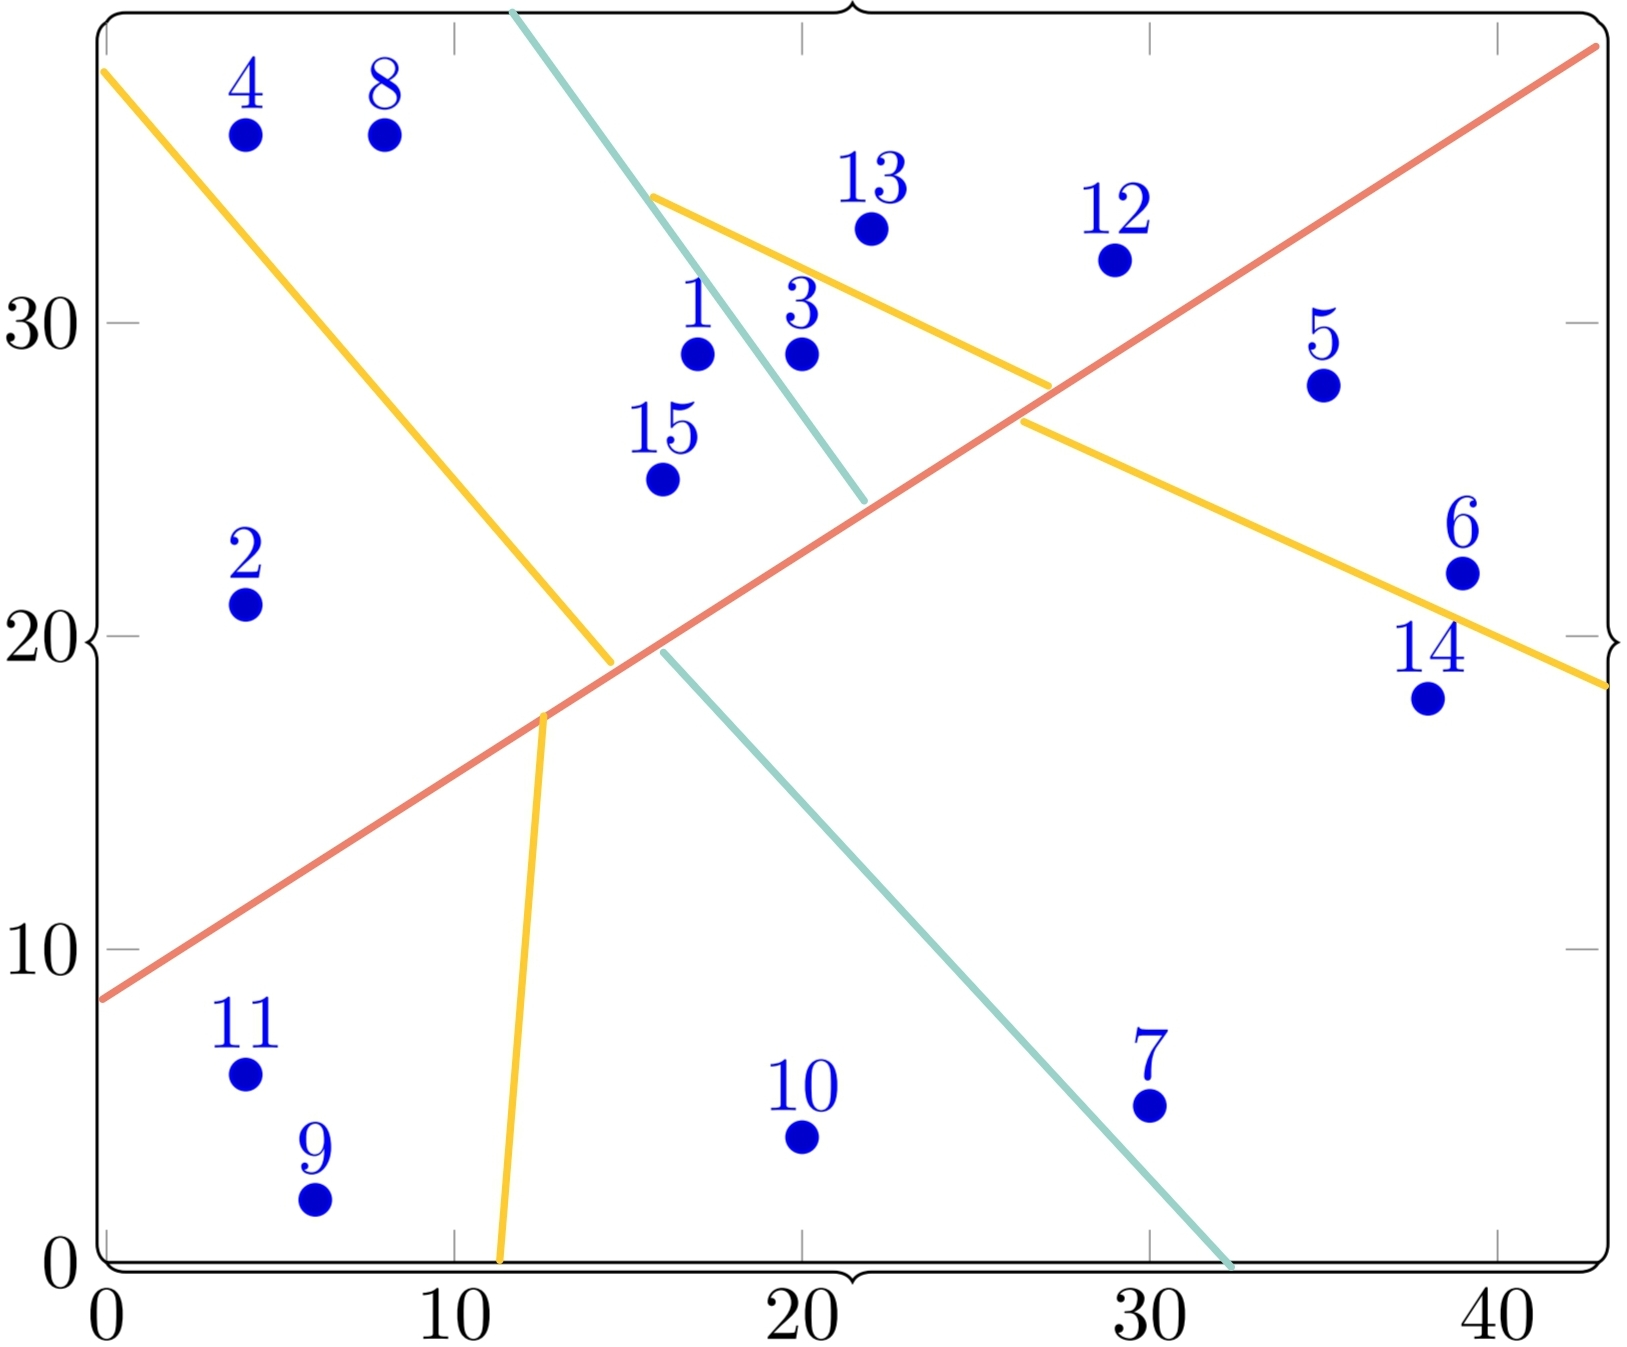
\includegraphics[scale = 0.15]{31drawing.jpg}
    \end{figure}

\item \textbf{VP Tree:}
Given the following VP tree, search for query point (25,4) with $\varepsilon = 11$.
Describe which parts of the tree you pruned and why.

\begin{center}
  \begin{tikzpicture}[every text node part/.style={align=center},level 1/.style={sibling distance=60mm},level 2/.style={sibling distance=30mm},level 3/.style={sibling distance=15mm}]
\node { 7\\(30, 5)\\$r=26.01$ } child {node { 14\\(38, 18)\\$r=21.95$ } child {node { 6\\(39, 22)\\$r=13.73$ } child {node { 5\\(35, 28) }} child {node { 3\\(20, 29) }}} child {node { 15\\(16, 25)\\$r=23.23$ } child {node { 10\\(20, 4) }} child {node { 9\\(6, 2) }}}} child {node { 1\\(17, 29)\\$r=13.57$ } child {node { 8\\(8, 36)\\$r=17.85$ } child {node { 13\\(22, 33) }} child {node { 12\\(29, 32) }}} child {node { 4\\(4, 36)\\$r=22.5$ } child {node { 2\\(4, 21) }} child {node { 11\\(4, 6) }}}};
  \end{tikzpicture}
  \end{center}

{\bf Solution:}\\
The Euclidean distance formula for calculating distance between two co-ordinates $(x_1,y_1)$ and $(x_2,y_2)$ are


\[ d(p,q) = \sqrt{(x_2-x_1)^2+{(y_2-y_1)^2}} \]

We have to define if we want to go through the left sub-tree or right sub-tree.
Formula for calculating the left sub-tree is 
\[ {max\{d(p,q)-r,0\} \le \epsilon } \]

Formula for calculating the right sub-tree is
\[ {max\{r-d(p,q),0\}  \le \epsilon } \]


\begin{itemize}
    \item Distance between Root node \textbf{7:(30,5) and Query point (25,4)} with $r = 26.01$ and $\epsilon = 11$

\[ d(p,q) = \sqrt{(25-30)^2+{(4-5)^2}} = 5.09 \le 11 \quad \textbf{Add the node to tree} \] 
    Verifying if we should go through left sub-tree
    \[d(7,q)-r = 5.09-26.01 = -20.91 \]
    \[ {max\{d(p,q)-r,0\} \le \epsilon} = {max\{d(7,q)-r,0\} = max\{-20.91,0\}} \le 11 \quad \textbf{Go through left sub-tree} \]
    
    Verifying if we should go through right sub-tree
     \[r-d(7,q) = 26.01-5.09 = 20.92 \]
    \[ {max\{r-d(p,q),0\}  \le \epsilon } = {max\{,0\} = max\{20.92,0\}} \nleq 11 \quad  \textbf{Prune right sub-tree}\] 

    \textbf{Now we only consider the co-ordinates of the left sub-tree for the query point as we have pruned the right sub-tree}
\\
    
    \item Distance between \textbf{14: (38,18) and Query point (25,4)} with r = 21.95 and $\epsilon = 11$


    \[ d(14,q)= 19.10 \nleq 11 \quad \textbf{don't add node } \]

    Verify left sub-tree \[ max\{-2.84,0\} = 0 \le 11 \quad \textbf{ traverse through the left sub-tree}\]
    Verify right sub-tree \[ max\{2.85,0\} = 2,85 \le 11 \quad \textbf{ traverse through the right sub-tree}\]

    \item Distance between \textbf{6: (39,22) and Query point (25,4)} with $r = 13.73$ and $\epsilon = 11$

     \[ d(6,q)= 22.80 \nleq 11 \quad \textbf{don't add node } \]
     
    Verify left sub-tree \[ max\{9.52,0\} = 9.52 \le 11 \quad \textbf{ traverse through the left sub-tree}\]
    Verify right sub-tree \[ max\{-9.07,0\} = 0 \le 11 \quad \textbf{ traverse through the right sub-tree}\]

    \item Distance between \textbf{15: (16,25) and Query point (25,4)} with r = 23.23 and $\epsilon = 11$

     \[ d(15,q)= 22.84 \nleq 11 \quad \textbf{don't add node } \]
     
    Verify left sub-tree \[ max\{0.89,0\} = 0 \le 11 \quad \textbf{ traverse through the left sub-tree}\]
    Verify right sub-tree \[ max\{0.39,0\} = 0 \le 11 \quad \textbf{ traverse through the right sub-tree}\]

    \item Distance between \textbf{5: (35,28) and Query point (25,4)} $\epsilon = 11$

     \[ d(5,q)= 26 \nleq 11 \quad \textbf{don't add node } \]

     \item Distance between \textbf{3: (20,29) and Query point (25,4)} $\epsilon = 11$

     \[ d(3,q)= 25.49 \nleq 11 \quad \textbf{don't add node } \]

     \item Distance between \textbf{10: (20,4) and Query point (25,4)} $\epsilon = 11$

     \[ d(10,q)= 5 \leq 11 \quad \textbf{ add node } \]

      \item Distance between \textbf{9: (6,2) and Query point (25,4)} $\epsilon = 11$

     \[ d(6,q)= 19.10 \nleq 11 \quad \textbf{don't add node } \]


     Hence \textbf{7 and 10 } nodes would be added to the result.
\end{itemize}
\end{enumerate}

\end{document}
